%------------------------------------------------------------------------------
% Planning
%------------------------------------------------------------------------------

\subsection{Planning}

The CowHub project started with very open-ended objectives, as seen above. Clearly, focused and specific planning was required. For the first week of the project we sought to narrow down exactly what this project meant and hoped to achieve, and the resulting week-long sprint proved highly successful and we realised the following:

\begin{itemize}
	\item We needed to delegate our responsibilities, between front-end interfaces and for back-end services
	\item The pivot point in our project would be a central, open API which would provide the backbone between our public and private services
	\item We needed to use stable, durable systems with sufficient amounts of compute power available, and link these with a solid continuous integration and deployment system
\end{itemize}

Owing to the abstract and preliminarily unidentified technical objectives of the project, a significant part of our team work and organisation has been to evolve the project description and iteratively redefine it. Consequently, we have seen various unanticipated changes in both infrastructure and 

%------------------------------------------------------------------------------
% Group organisation
%------------------------------------------------------------------------------

\subsection{Group Organisation}

In the beginning, the group members allocated each other responsibilities to give the project direction and a clear starting point for each member. As a group we decided on fundamental requirements for each component which was the only specification for each microservice / interface. The group agreed that we would spend as little time as possible in a horizontal development stage, and by parallelising the bootstrapping of the project, we were able to quickly reach a position where we could employ strong software engineering practices to maintain a high level of productivity. The responsibilities we each started with are below:

\begin{itemize}
	\item	\textbf{Frederick Lindsey, Gregoire Yharrassarry, Karim Nahas} \\
		  	Initial web front-end and basic API gateway, providing stateless session management, and performant asynchronous access to back-end services. 
		  	Bootstrapping the React-Redux web front-end and Ruby-on-Rails API gateway repositories. Setting up continuous integration and deployment for these repositories.
	\item 	\textbf{Thomas Szyszko} \\
		  	Investigated and implemented a portable mobile platform which could be used to input cattle information and identify cattle.
		  	Initialised and bootstrapped a Cordova-based application.
	\item 	\textbf{Hongjiang Liu} \\
	 	  	Researched and implemented an algorithm to process an image into keypoints used for comparison to provide functionality determining how similar images and their textures are.
	 	  	Extensive research into best practices for understanding images (machine-wise) and their differences.
\end{itemize}

As the project progressed, the responsibilities we each had became more and more general and translated across the platform. The group became very adaptable as the depth of each member's knowledge grew and we could all pick up any task on most components. The group had great flexibility when different members time constraints changed and was able to maintain a constant level of progress throughout the project resulting in a project that has been consistently worked on for three months. Crucial to this was meeting on a regular basis and maintaining persistent communication largely in the form of online communication and note-taking.

Towards the end of the project, due to time constraints, we reduced the breadth of the front-end footprint in order to focus on the core algorithm and infrastructure improvement to best achieve our directives and objectives.

%------------------------------------------------------------------------------
% Breakdown and task allocation
%------------------------------------------------------------------------------

\subsection{Breakdown and Task Allocation}

During the course of the project, the group experienced a myriad of changes to the way in which we managed ourselves and the tools we used. This allowed us to continually improve our productivity potential all whilst learning the ins and outs of real-world software engineering and development.

\subsubsection{Tracking tasks and issues}

Central to any software development is a teams ability to accurately, and in real-time, track what they are doing, what they need to do, and what they have achieved. The team adopted the Kanban approach, suggesting feature requests and issues onto a backlog, and dedicating resources to each task (often a user story) such that we maintained constant progress through the board. We used columns including 'Backlog', 'In Progress', 'Review', 'Done',  'Blocked' and 'Ignored' throughout our project to monitor tasks and be able to evaluate our performance as a team.

The first tool we tried to use to implement our chosen style of development was Trello \footnote{\href{https://trello.com}{Trello} provides an online workspace especially designed for todos and task management using cards.}

\begin{figure}[H]
	\centering
	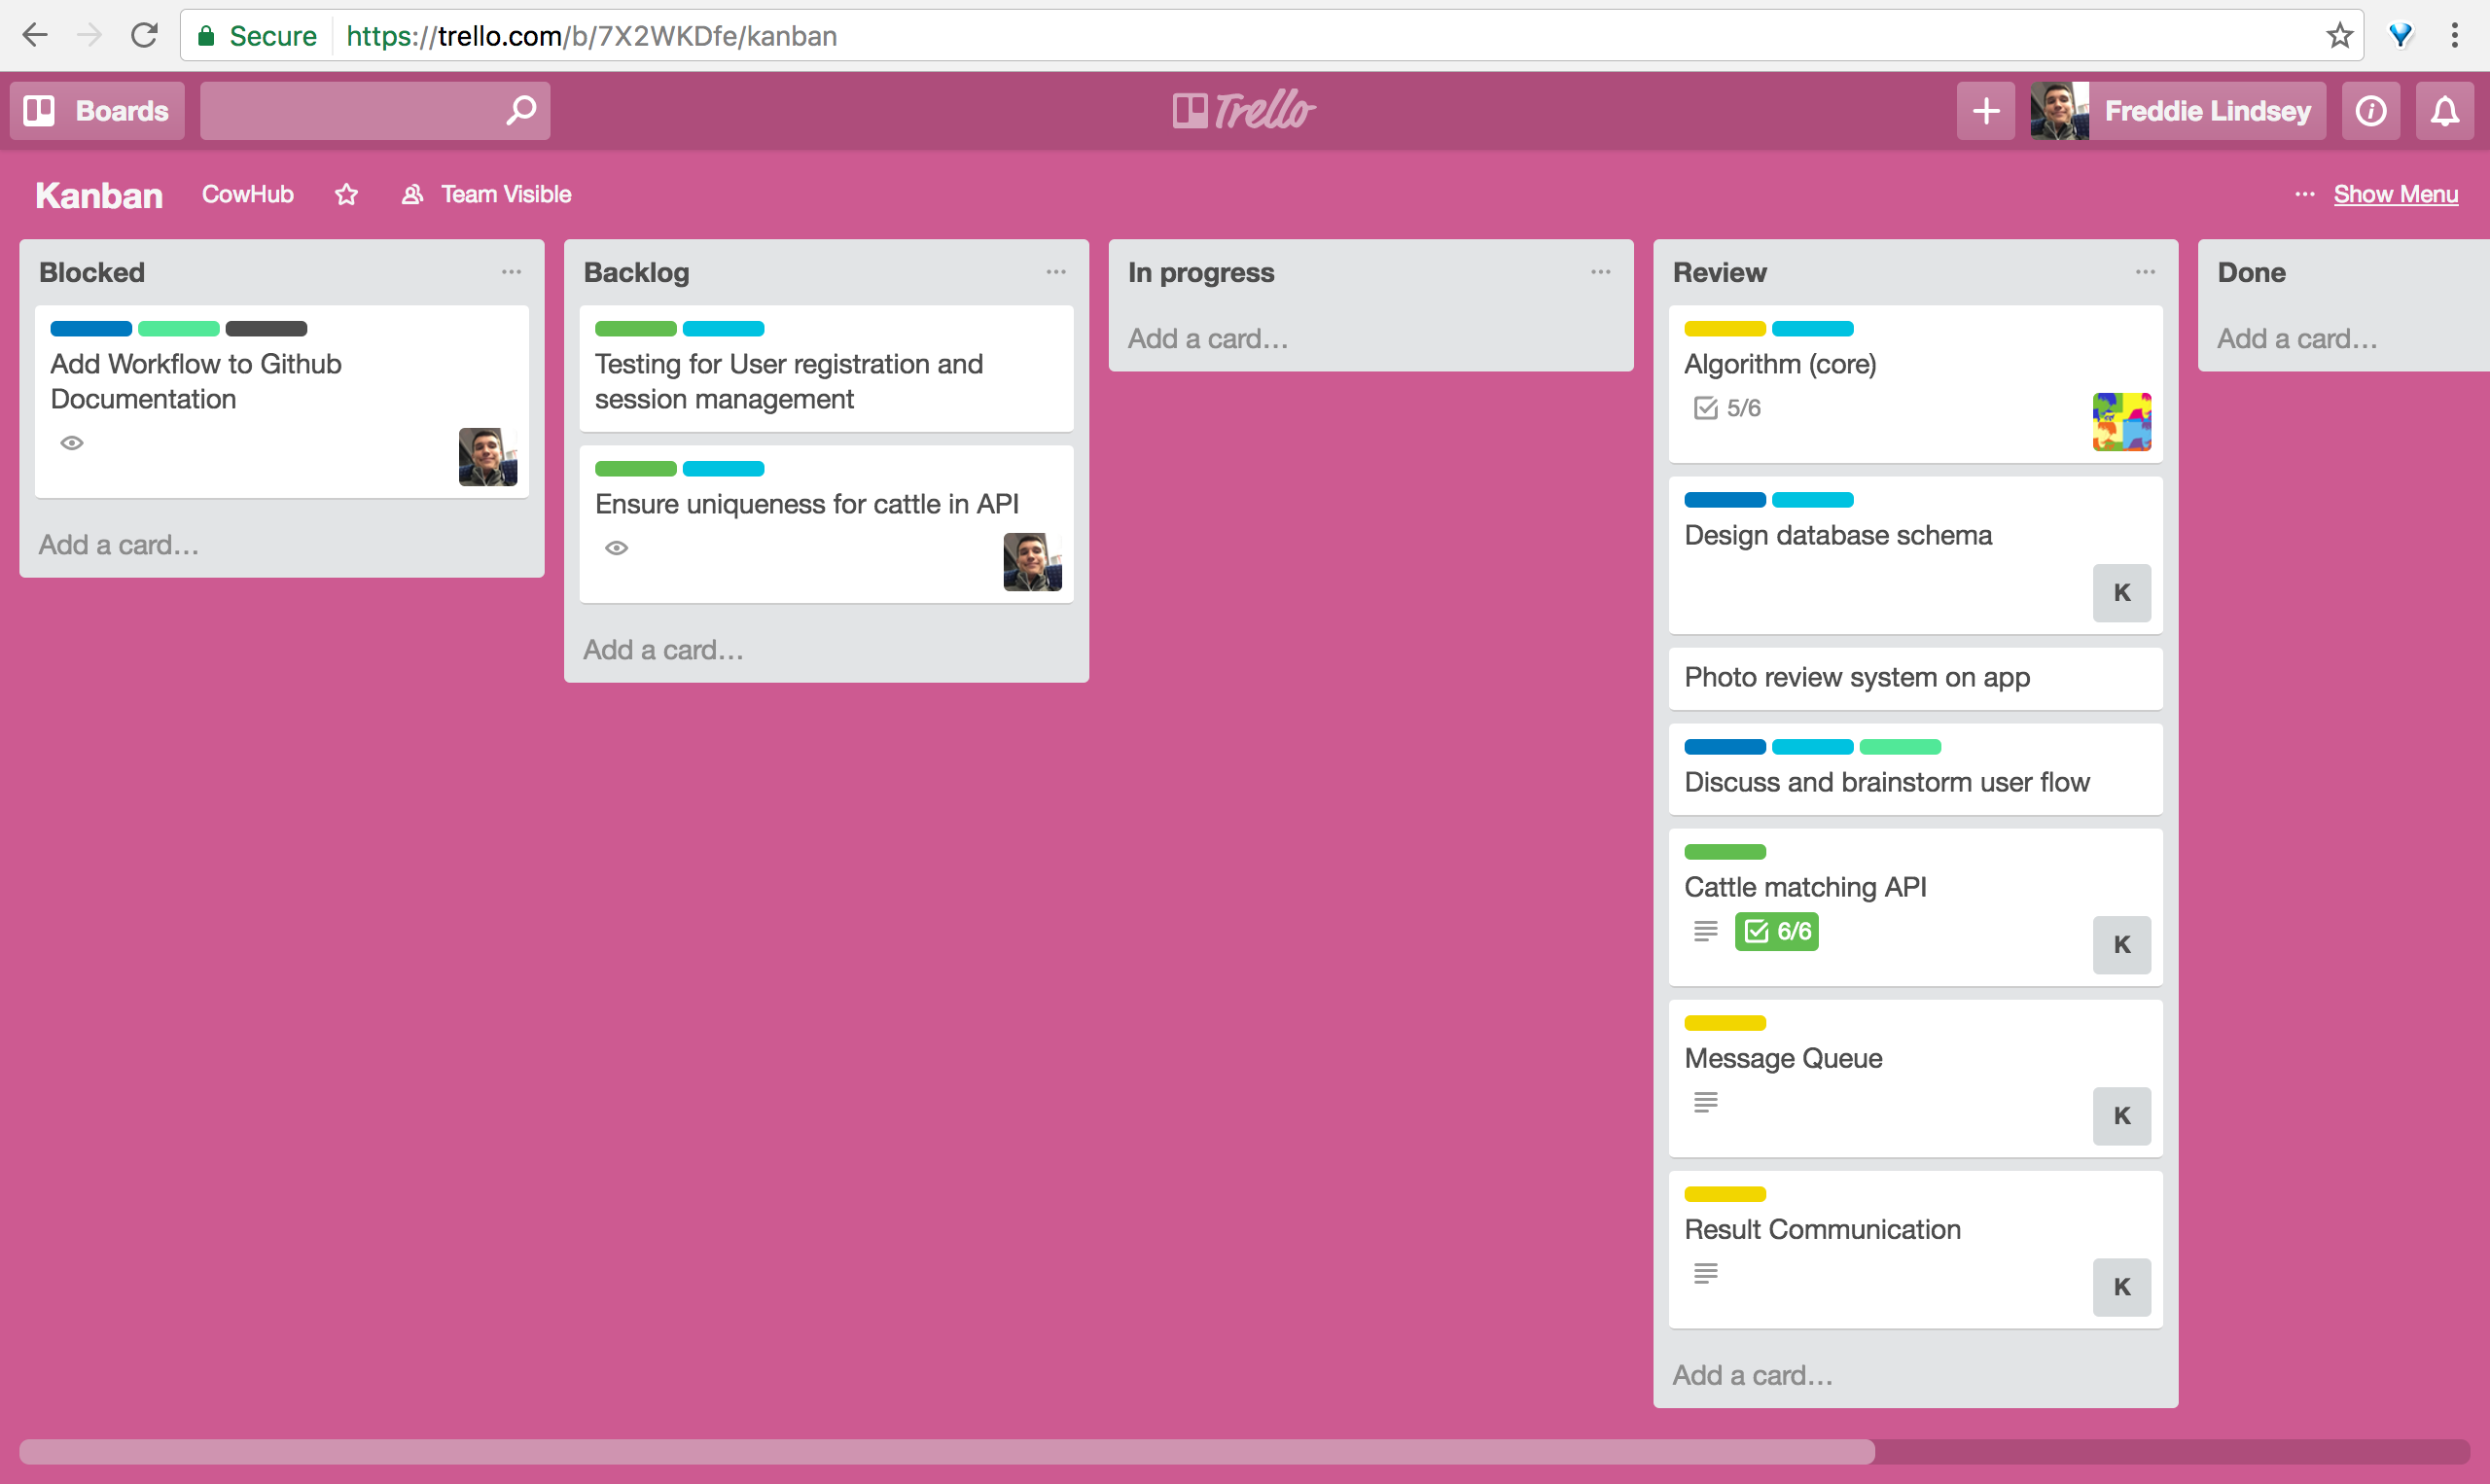
\includegraphics[width=0.8\textwidth]{images/trello-kanban}	
	\caption[CowHub's 'Kanban' board on Trello]{
		Our preliminary tool for tracking our tasks and issues, emulating the infamous Kanban approach.
	}
\end{figure}

During the limited time we chose to use Trello, we discovered that it made our development process more difficult, not easier as we had hoped and anticipated. The core reason for this was the separation between how we managed what tracking what we were doing (Trello), and actually managing the what we were doing itself (GitHub/GitLab). This separation, and the extra effort required to manage ourselves resulted in very low usage of the board, and no benefit to our workflow.

Consequently, we soon rejected Trello as our main tracking tool and instead reverted to using whiteboards whenever we met as a group and were working as a team. This was a great strategy whilst we were working, but we found that the ephemeral nature of the board was a hinderance to maintaining and keeping track of the project's progress.

As part of a wider transition from privately hosted servers to cloud infrastructure owned and serviced by a public company \footnote{We used AWS for our final deployment, although we also considered Microsoft Azure amongst others}, we were able to use GitHub for cloud-hosted version control. This gave us the chance to be able to tie in our version control and task management in the same window. This radically improved our efficiency when managing what we were each developing and contributing to and raised our productivity levels dramatically. A sample of our Kanban-esque board on GitHub Projects is shown below.

\begin{figure}[H]
	\centering
	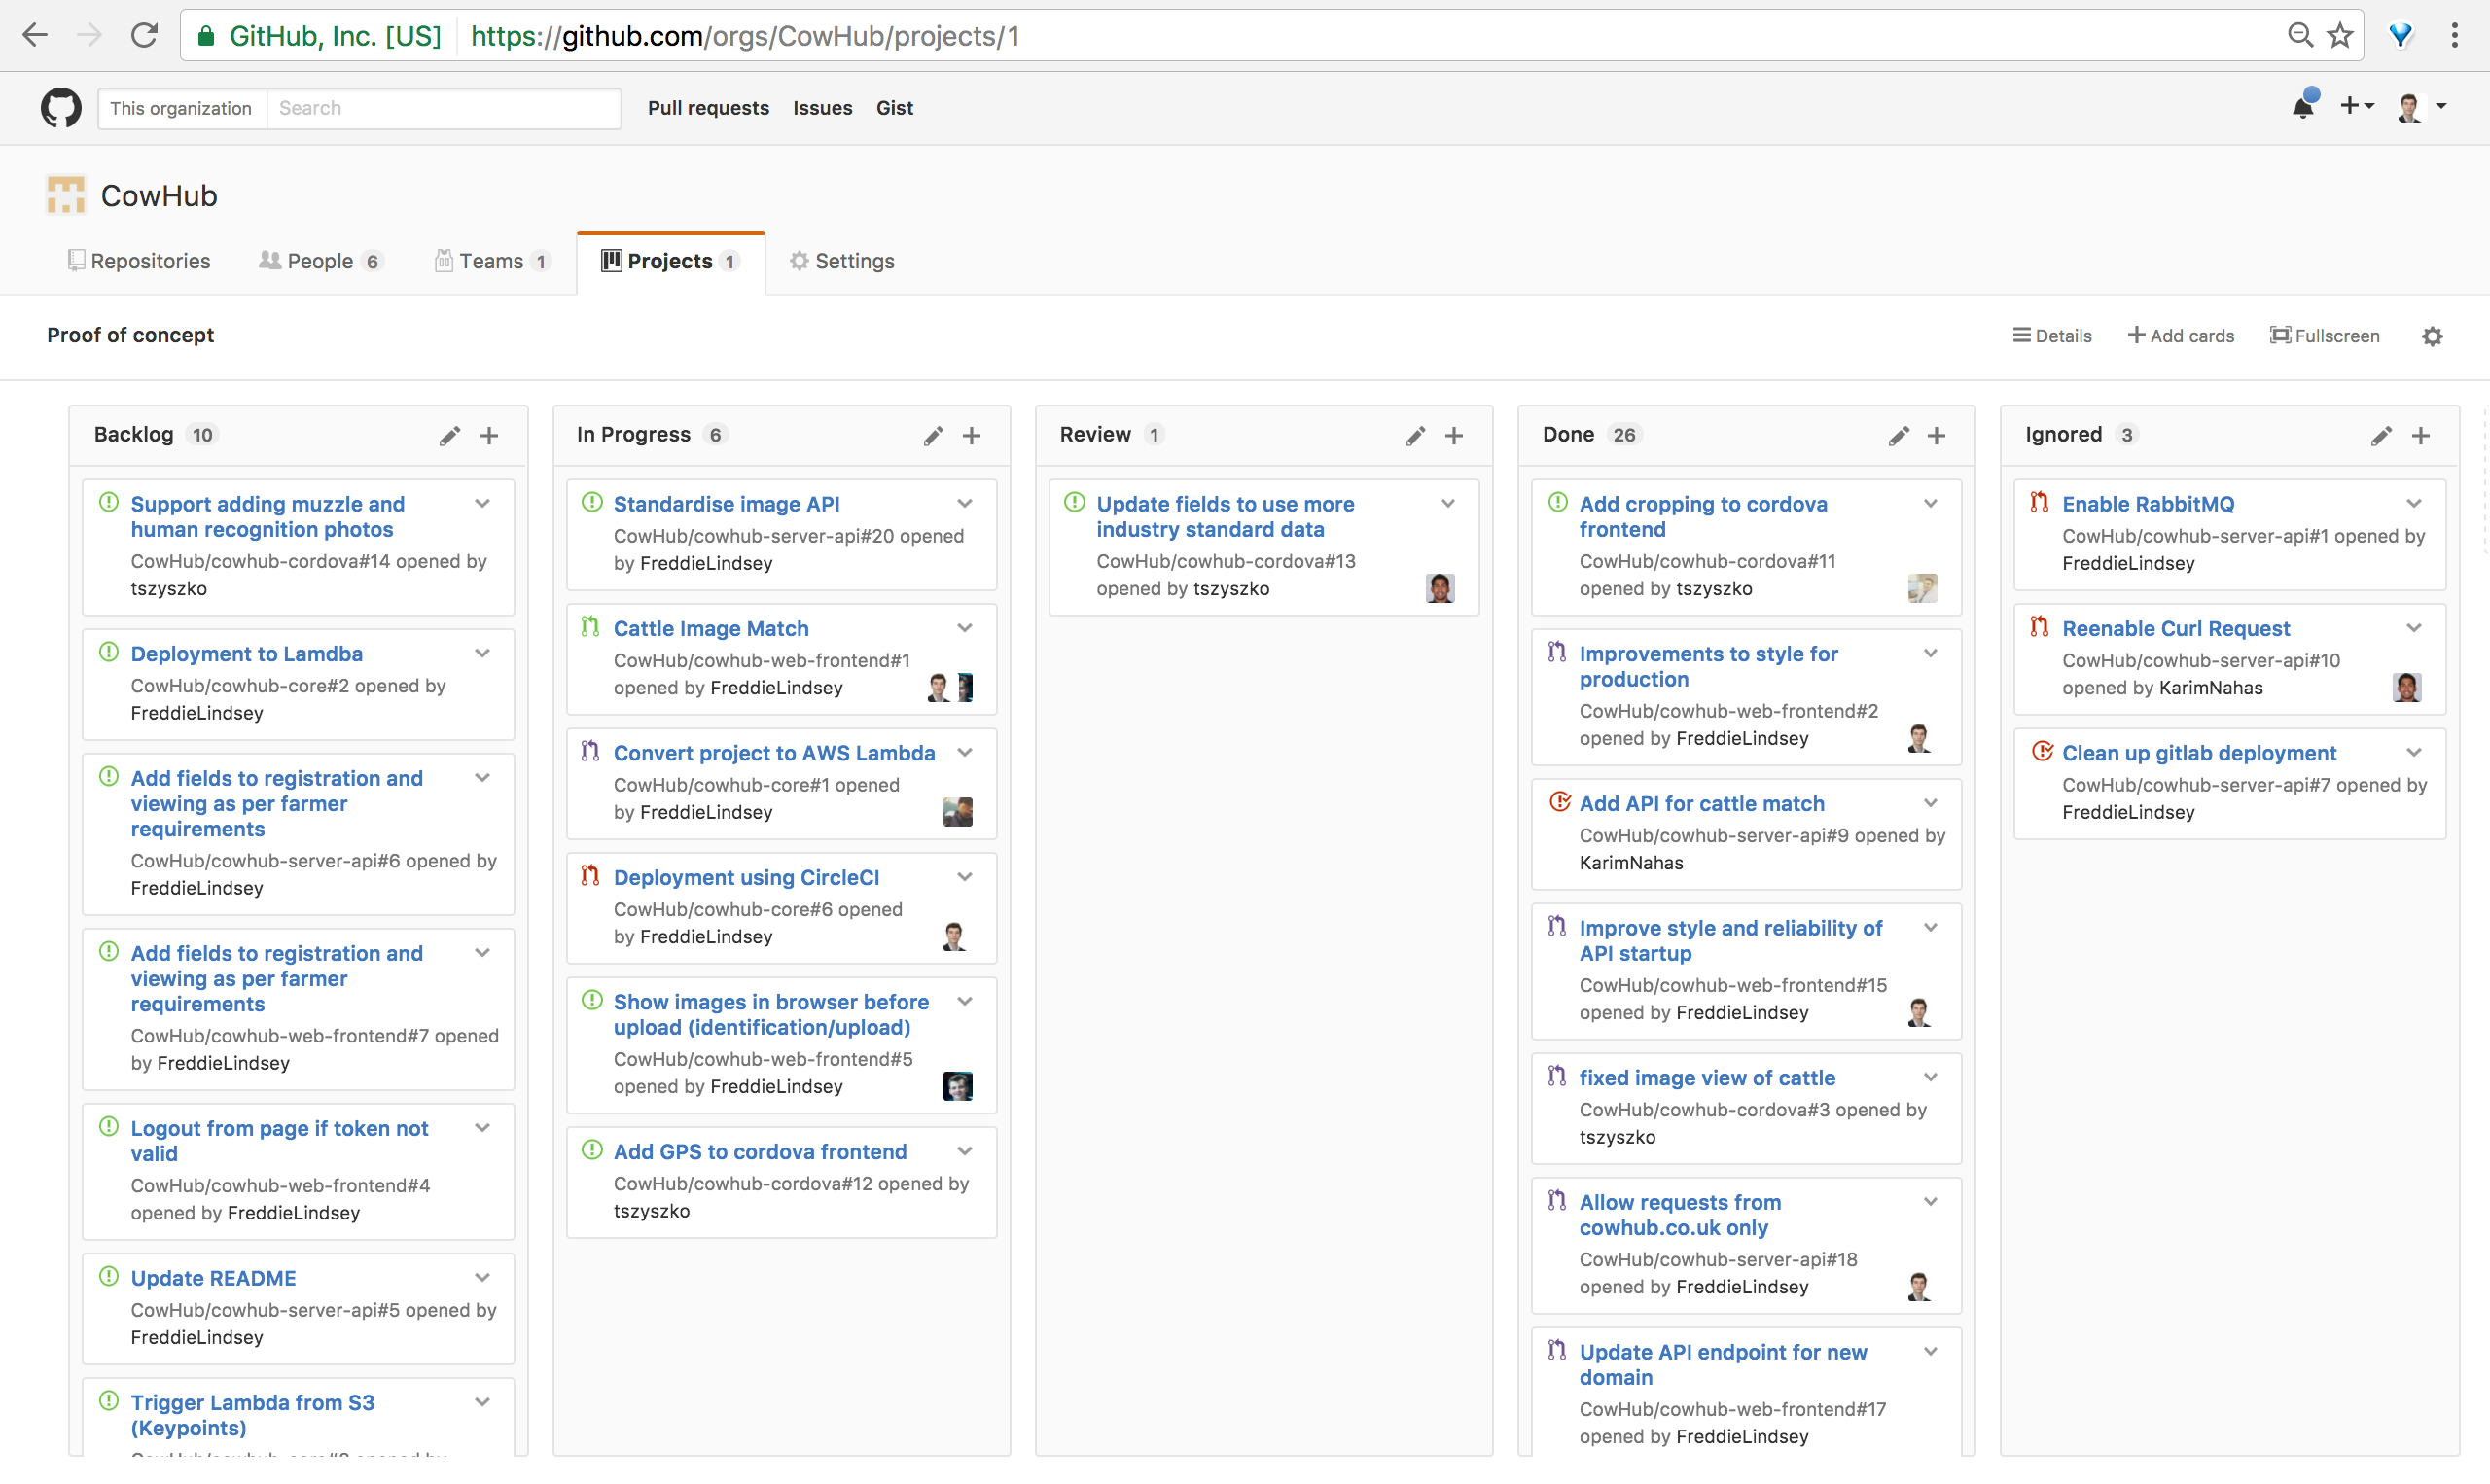
\includegraphics[width=0.8\textwidth]{images/github-project}
	\caption[CowHub's 'Kanban' board on GitHub using GitHub Projects]{
		A display of part of our board on GitHub, showing icons to determine the type of card
	}
\end{figure}


\subsubsection{Communication}







